% Short paper draft for Geophysical Journal International (GJI).
% Compiles with pdflatex + bibtex using the standard `article` class so it
% builds anywhere; to submit, swap in the GJI class (\documentclass{gji}) and
% move the abstract into the \begin{summary} environment.
\documentclass[11pt]{article}

\usepackage[margin=1in]{geometry}
\usepackage{graphicx}
\usepackage{amsmath}
\usepackage{natbib}
\usepackage{xcolor}
\usepackage[hidelinks]{hyperref}
\usepackage{siunitx}

\graphicspath{{../literature/figs/}}
\bibliographystyle{abbrvnat}
\setcitestyle{authoryear,round}

\newcommand{\dvv}{\ensuremath{\delta v/v}}

\title{\textbf{Processing choices, not physics: the reproducibility cost of
ad-hoc decisions in ambient-noise seismic velocity-change monitoring}}

\author{M.~A.~Denolle\thanks{Department of Earth and Space Sciences, University
of Washington, Seattle, WA, USA. \texttt{mdenolle@uw.edu}} \quad
\textit{[co-authors TBD]}}

\date{Draft --- \today}

\begin{document}
\maketitle

\begin{abstract}
\noindent
Relative seismic velocity changes (\dvv) measured from the ambient seismic field
are now a standard monitoring observable for volcanoes, faults, landslides,
aquifers and the cryosphere. Yet the pipeline that turns cross-correlation
functions into a \dvv\ time series involves a long sequence of choices --- the
estimator, the frequency band, the coda window, the reference, the stacking, and
how cross-components and station pairs are aggregated and weighted --- that are
made \emph{ad hoc} and are seldom reported in full. Using a controlled synthetic
in which the ground-truth \dvv\ is known exactly, we quantify how much each
choice moves the recovered value \emph{and its stated uncertainty}. We reproduce
all seven estimators of the \textsc{NoisePy} monitoring toolbox and show that, at
large \dvv, methods split by family with distinct failure modes; that the same
station pair yields different \dvv\ time series depending only on whether one
averages the per-component \dvv\ or the correlation-coefficient images; and,
most consequentially, that the reported $1\sigma$ on a network-averaged \dvv\
varies by a factor of $\sim\!\sqrt{N}$ purely from the standard-error-versus-
standard-deviation and weighting conventions --- so a change that is
``$3\sigma$ significant'' in one study is ``not significant'' in another, from
identical data. We argue that these undocumented choices, not the physics, are
the leading obstacle to intercomparing \dvv\ studies, and we propose a minimal
reporting standard and an open, executable framework (\textsc{codameter}) that
makes every choice explicit and its effect reproducible.
\end{abstract}

\section{Introduction}
\label{sec:intro}

Coda-wave and ambient-noise interferometry measure relative changes in seismic
velocity, \dvv, by tracking the apparent stretching of late, multiply-scattered
arrivals between a reference and a current cross-correlation function
\citep{Snieder2002,SensSchonfelder2006}. Because the coda accumulates the
travel-time perturbation with lapse time, \dvv\ is exquisitely sensitive --- of
order $10^{-3}$ or smaller is routinely reported --- which is precisely why the
method has spread across volcano, fault-zone, landslide, hydrological and
cryospheric monitoring.

That sensitivity is a double-edged sword. The map from raw correlations to a
\dvv\ time series is long, and at almost every step the analyst makes a choice:
which estimator \citep{Yuan2021}, which frequency band and coda window (which
together set the sampled depth; \citealp{Obermann2013,Obermann2016}), which
reference \citep{Brenguier2014}, how much to stack, and --- the focus of the
second half of this paper --- how to aggregate and weight the many
cross-component and station-pair measurements that make up a network estimate.
These choices are typically made by habit, justified briefly if at all, and
rarely reported in enough detail to reproduce. The community has long flagged
\emph{individual} pitfalls (spurious changes from non-stationary noise,
\citealp{Zhan2013}; measurement-error formulae,
\citealp{Clarke2011,Weaver2011}), but the \emph{cumulative} effect of the full
choice set on both the value and its stated uncertainty has not been quantified
in one place.

This is a reproducibility problem of exactly the ``garden of forking paths''
type identified in the statistical sciences \citep{Gelman2013,Steegen2016}: many
individually defensible analyses of the same data give different answers, and
without pre-registration or full reporting the reader cannot tell signal from
choice. Here we make the problem concrete for \dvv\ monitoring. We build a
synthetic in which the truth is known, push it through the real estimators of an
open toolbox, and measure the artefact that each choice introduces. Our aim is
not to crown a ``best'' pipeline but to show that the choices are consequential,
that they are currently undocumented, and that the fix --- explicit reporting and
an executable record --- is cheap.

\section{A controlled synthetic framework}
\label{sec:methods}

We synthesize a reference coda cross-correlation function as a band-limited,
multiply-scattered wavefield with an exponentially decaying coda envelope, and
optionally a frequency-dependent decay $A(t)\propto e^{-\pi f t/Q_c}$ so that the
late coda fades first at high frequency. A homogeneous velocity change is
imposed exactly by stretching the lapse-time axis, $u_{\rm cur}(t) = u_{\rm
ref}\!\left(t/(1+\dvv)\right)$, and a daily time series is produced by repeating
this with a prescribed ground-truth $\dvv(t)$ and additive band-limited noise at
a controlled signal-to-noise ratio. Because the imposed $\dvv(t)$ is known, every
departure of a recovered series from it is an artefact of the processing, not of
the data.

We reproduce, live, all seven \dvv\ estimators of the \textsc{NoisePy}
\texttt{monitoring\_methods} module \citep{Jiang2020}: trace stretching (TS),
windowed cross-correlation (WCC), dynamic time warping (DTW), the moving-window
cross-spectrum (MWCS; \citealp{Clarke2011}), and three wavelet-domain methods
--- the wavelet cross-spectrum (WCS), wavelet stretching (WTS) and wavelet DTW
(WTDTW) --- benchmarked numerically by \citet{Yuan2021}. The wavelet methods use
a dependency-free Morlet continuous wavelet transform; WCS optionally unwraps the
cross-wavelet phase in two dimensions (along lapse, anchored at $\tau\!\to\!0$,
then along frequency) following \citet{Mao2020}. The framework, the figures
below, and a unit-tested implementation are released in the open
\textsc{codameter} package (Section~\ref{sec:discussion}).

\section{Results}
\label{sec:results}

\subsection{Estimator family}
\label{sec:methods-fig}

On small, clean \dvv\ all seven estimators sit on the one-to-one line
(Fig.~\ref{fig:methods}a): the choice is invisible and the result reproducible.
The choice bites at large \dvv\ (Fig.~\ref{fig:methods}b), where the methods
split by family. The stretching family (TS, WTS) and WCC match the whole dilated
coda and remain accurate; the phase methods read a wrapped phase, so MWCS
cycle-skips, while the \emph{same} cross-wavelet phase, once unwrapped in 2-D,
recovers the change --- success or failure turning on the unwrapping sub-choice
alone. The warping methods (DTW, WTDTW) track but under-shoot the largest
strains. No estimator is simply ``right''; an undocumented estimator choice
silently changes the answer once \dvv\ leaves the small-amplitude regime.

\begin{figure}[t]
  \centering
  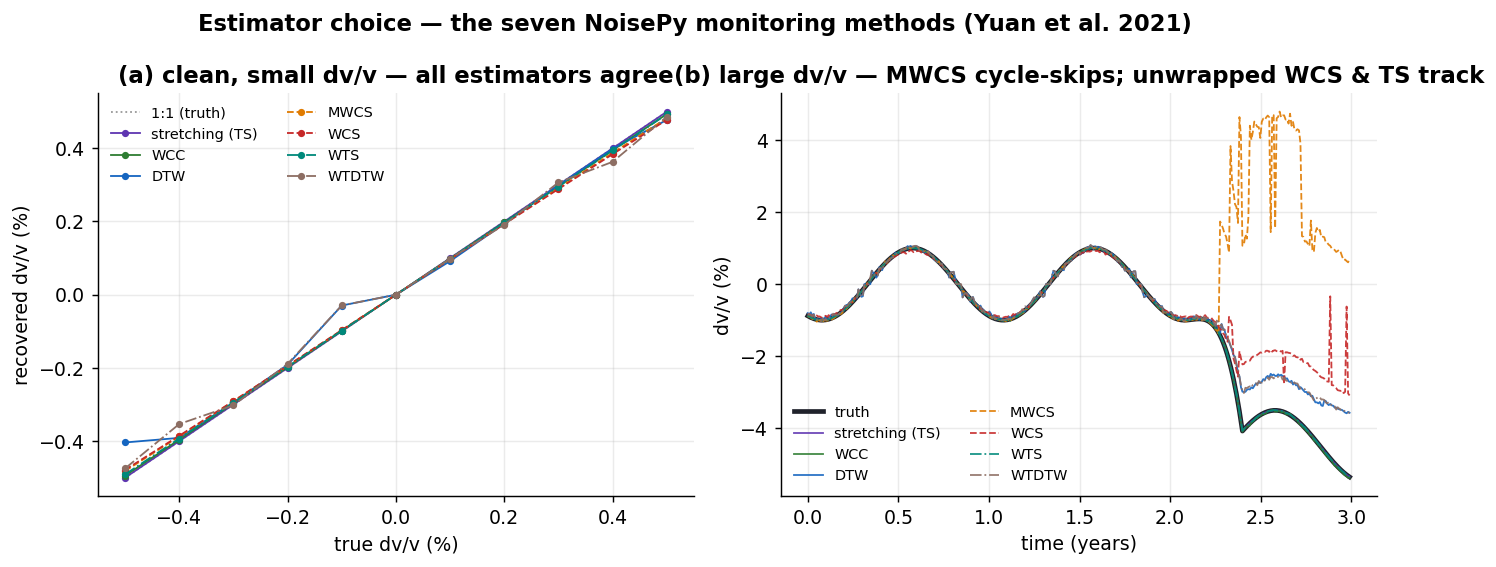
\includegraphics[width=\textwidth]{demo_1_methods.png}
  \caption{Estimator choice across the seven \textsc{NoisePy} methods. (a) Clean,
  small \dvv: all agree. (b) Large \dvv\ (a pre-failure landslide signal): MWCS
  cycle-skips, 2-D-unwrapped WCS and the stretching family track, the warping
  methods under-shoot.}
  \label{fig:methods}
\end{figure}

\subsection{Aggregating cross-components}
\label{sec:aggregation}

A single station pair carries several cross-component correlation functions, each
a noisy view of the same \dvv. How they are combined is a workflow choice that is
almost never reported, yet it changes both the value and the uncertainty
(Fig.~\ref{fig:aggregation}). One may peak-pick each component's correlation-
coefficient curve $\mathrm{CC}(\varepsilon,t)$ and then average the per-component
\dvv\ (Approach A) --- unweighted, a few poor components drag the mean around;
coherence-weighted, they are suppressed --- or one may average the
$\mathrm{CC}(\varepsilon,t)$ \emph{images} across components first and peak-pick
once (Approach B). All three recipes appear in the literature; on the same pair
they give visibly different time series, and they propagate uncertainty along
incompatible pathways (the ensemble spread of the per-component picks for A, the
width of the averaged correlation peak for B).

\begin{figure}[t]
  \centering
  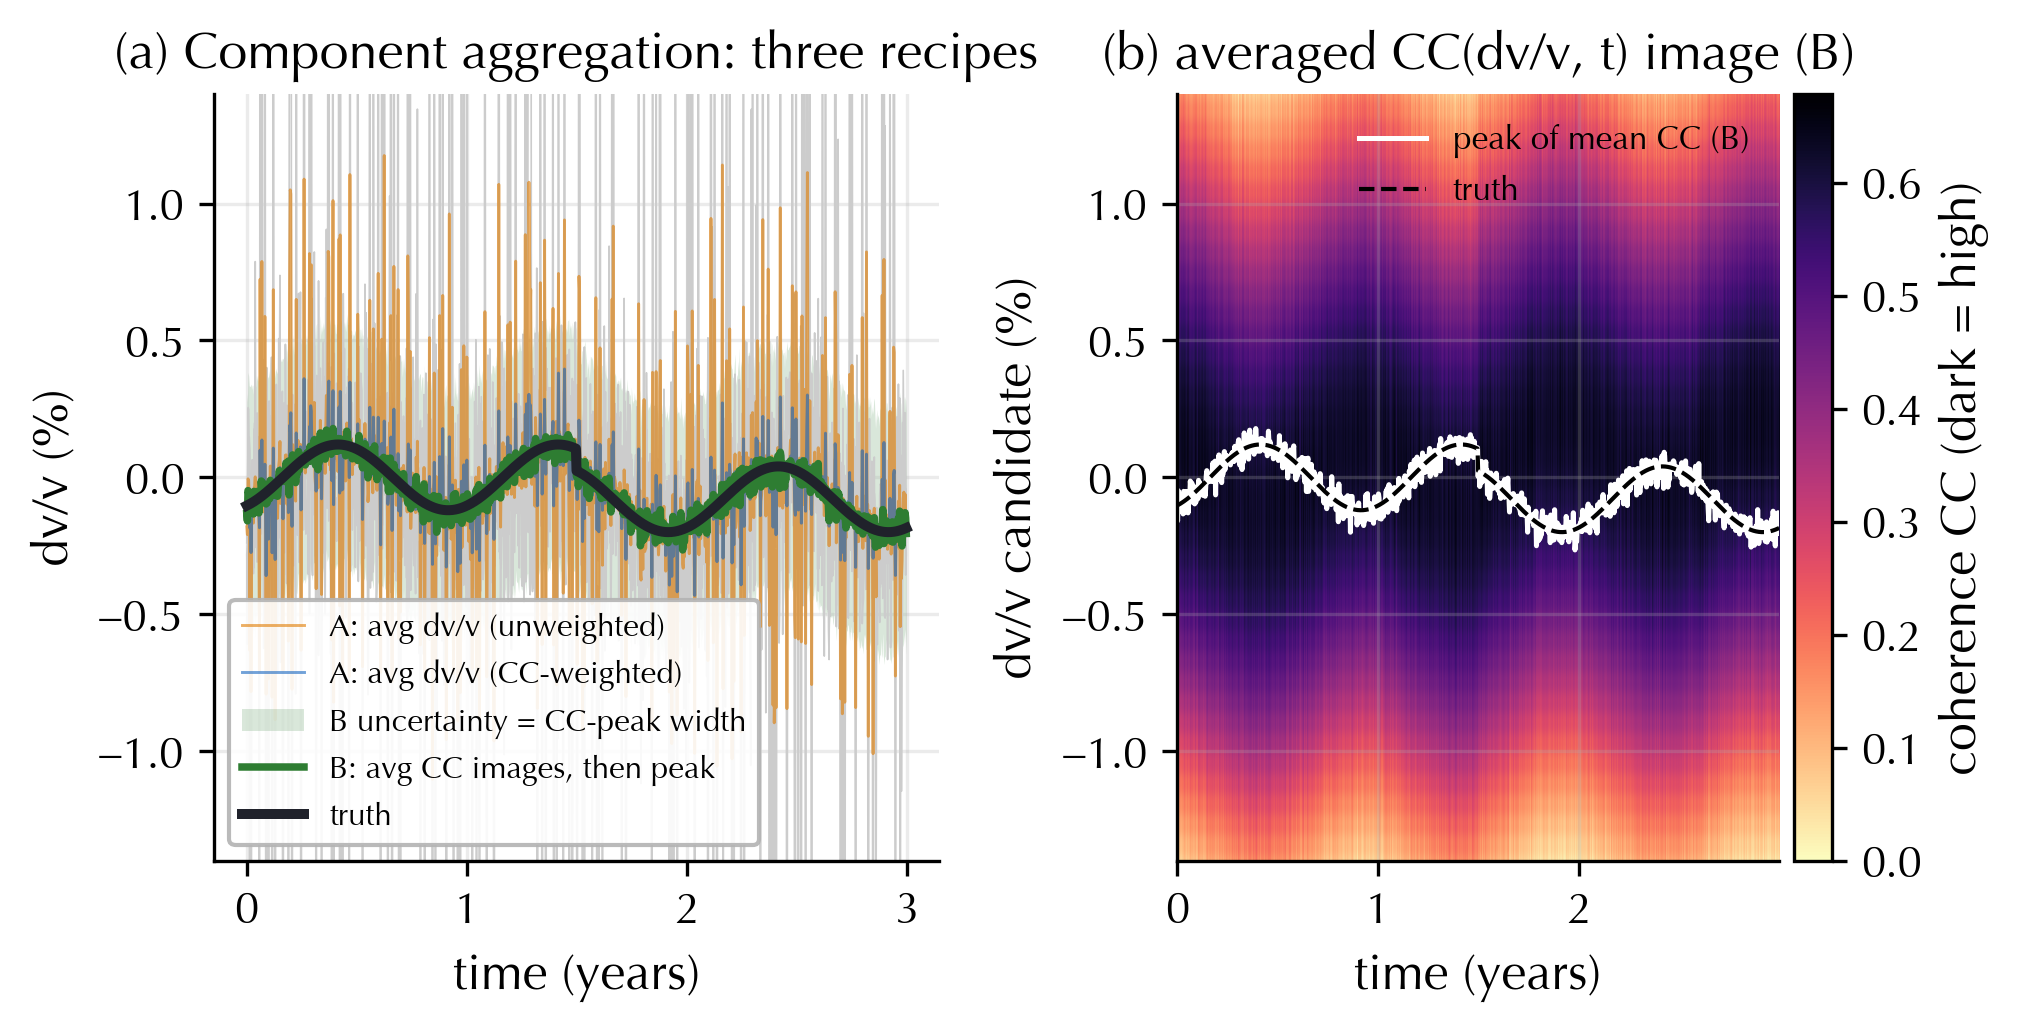
\includegraphics[width=\textwidth]{demo_2_aggregation.png}
  \caption{Cross-component aggregation for one station pair. (a) Unweighted
  \dvv-averaging swings with the poor components, while coherence-weighting and
  image-averaging track the truth. (b) The averaged $\mathrm{CC}(\dvv,t)$ image
  of Approach B with its peak ridge.}
  \label{fig:aggregation}
\end{figure}

\subsection{Network aggregation and the reported error bar}
\label{sec:uncertainty}

Adding the next layer up --- combining many station pairs into a network series
--- exposes the most consequential and least-reported choice of all: how to
summarize the uncertainty. Three conventions are common: a coherence-weighted
standard error, an unweighted standard error ($\sigma=\mathrm{std}/\sqrt{N}$),
and the between-pair standard deviation (the scatter, \emph{not} divided by
$\sqrt{N}$). On the same synthetic network the recovered means nearly coincide,
but the reported $1\sigma$ spans a factor of $\sim\!\sqrt{N}$
(Fig.~\ref{fig:uncertainty}). A velocity change that is ``$3\sigma$ significant''
under the tightest convention is ``$1\sigma$, not significant'' under the most
conservative one --- from identical data. Error bars on published \dvv\ are
therefore not comparable across studies unless the aggregation, the weighting,
and the standard-error-versus-standard-deviation convention are all stated.

\begin{figure}[t]
  \centering
  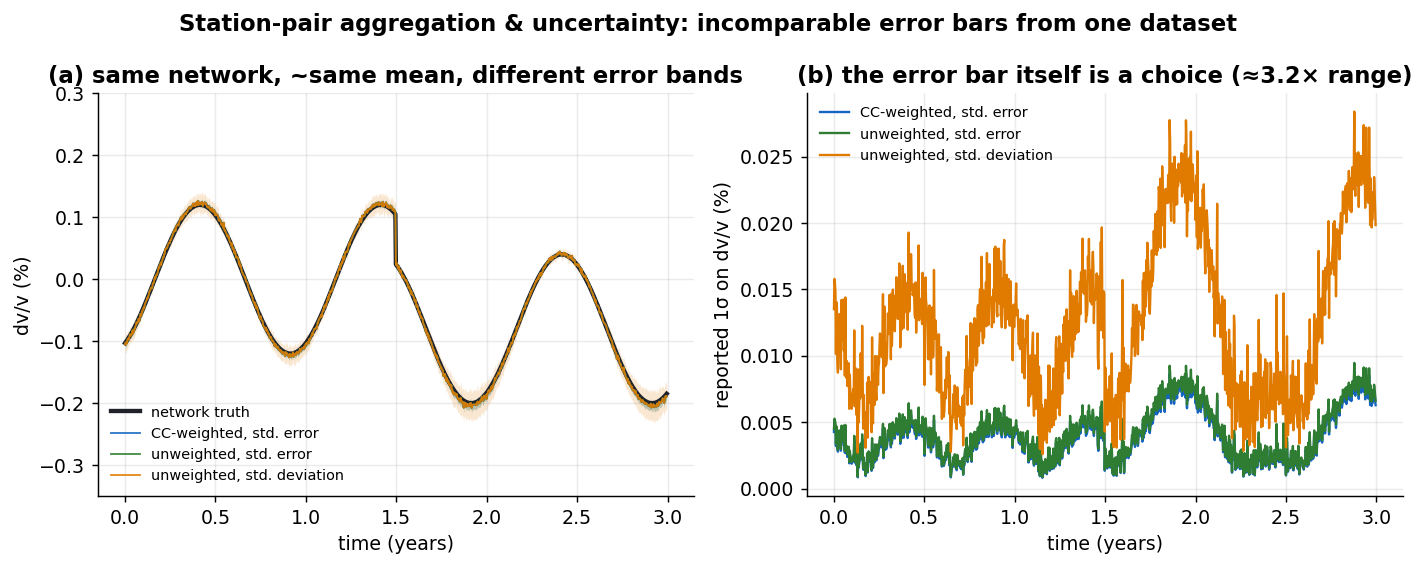
\includegraphics[width=\textwidth]{demo_3_uncertainty.png}
  \caption{Station-pair aggregation and uncertainty for a nine-pair network. (a)
  The recovered \dvv\ agrees across conventions; the shaded $1\sigma$ bands do
  not. (b) The reported $1\sigma$ differs by $\sim\!\sqrt{N}$ purely from the
  weighting and SE-versus-SD choices.}
  \label{fig:uncertainty}
\end{figure}

\subsection{Frequency band, coda window, reference and stacking}
\label{sec:params}

The remaining choices are no less consequential. The frequency band sets the
sampled depth: in a two-layer medium, banding high recovers a shallow seasonal
signal and banding low recovers a deep trend --- the band chooses \emph{what is
measured} (Fig.~\ref{fig:params}a). The coda window does not transfer across
bands: because the coda fades first at high frequency, a late window that is full
of signal at low frequency is pure noise at high frequency, and reusing it
returns garbage (Fig.~\ref{fig:params}b). The reference defines what survives: a
moving reference re-baselines continuously and erases slow trends that a fixed
reference or a joint inversion \citep{Brenguier2014} preserve
(Fig.~\ref{fig:params}c). And the stacking length trades noise against temporal
resolution, rounding off and delaying a coseismic step (Fig.~\ref{fig:params}d).

\begin{figure}[t]
  \centering
  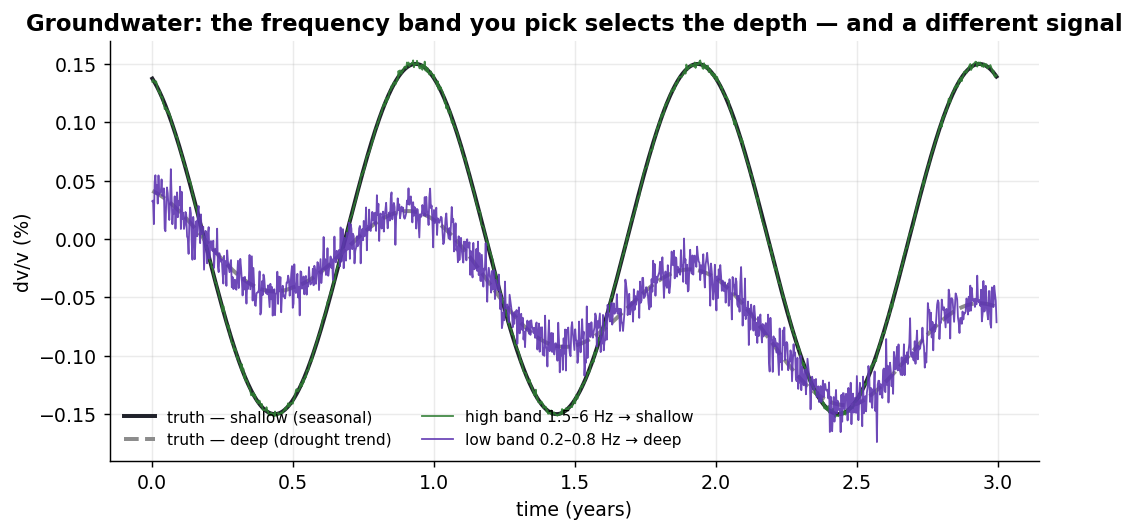
\includegraphics[width=0.49\textwidth]{demo_4_frequency_depth.png}\hfill
  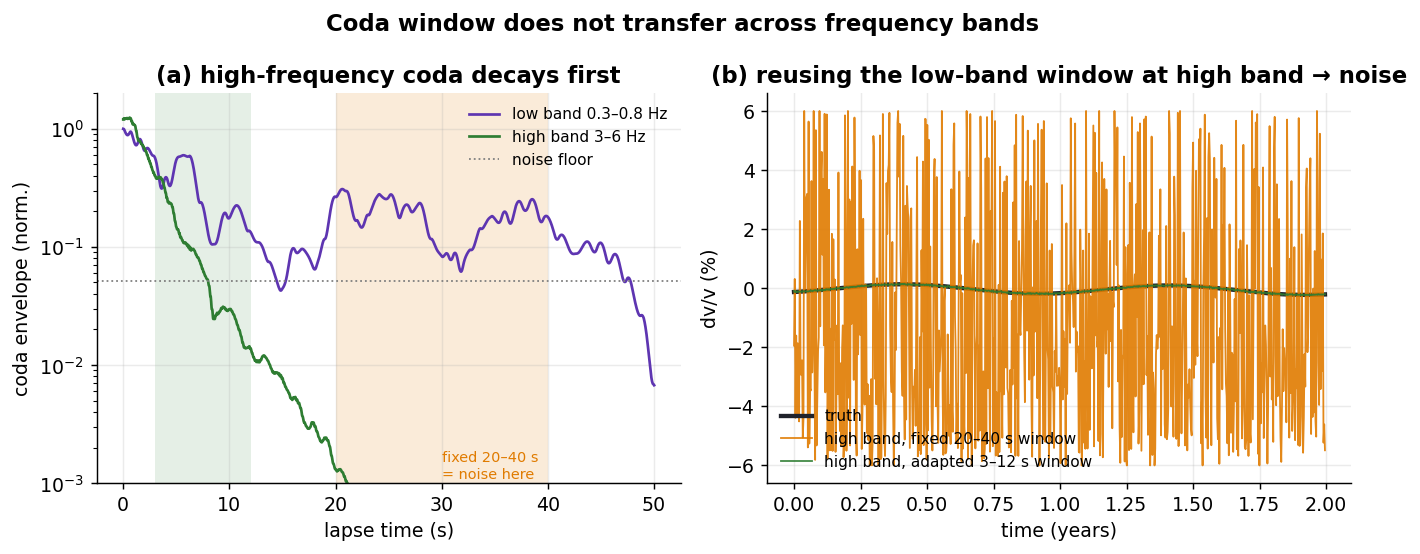
\includegraphics[width=0.49\textwidth]{demo_5_window_band.png}\\[2pt]
  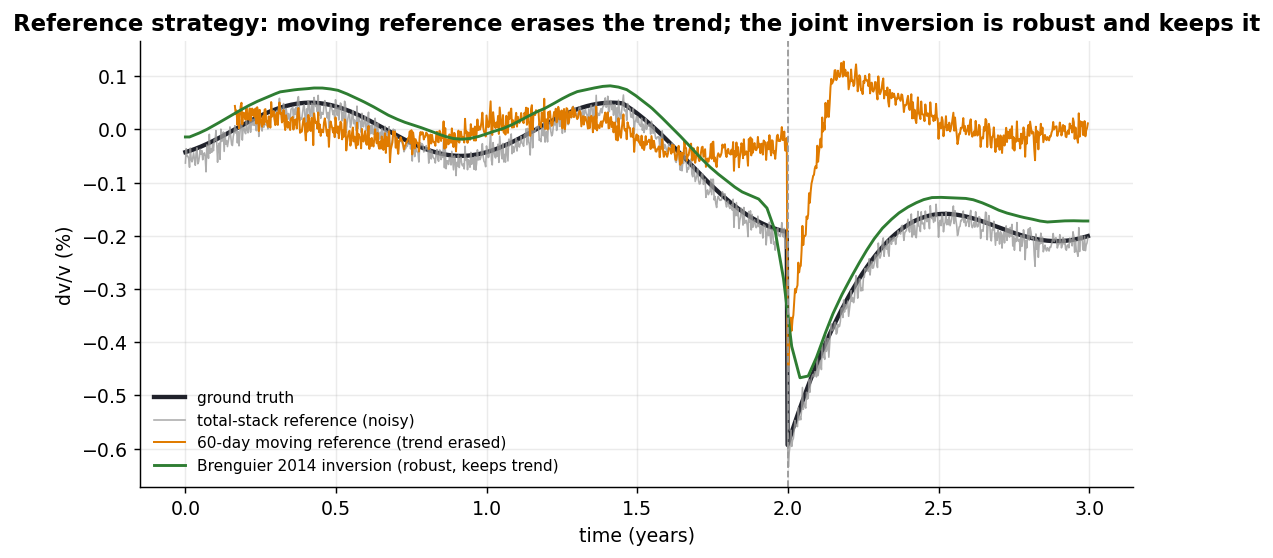
\includegraphics[width=0.49\textwidth]{demo_7_reference.png}\hfill
  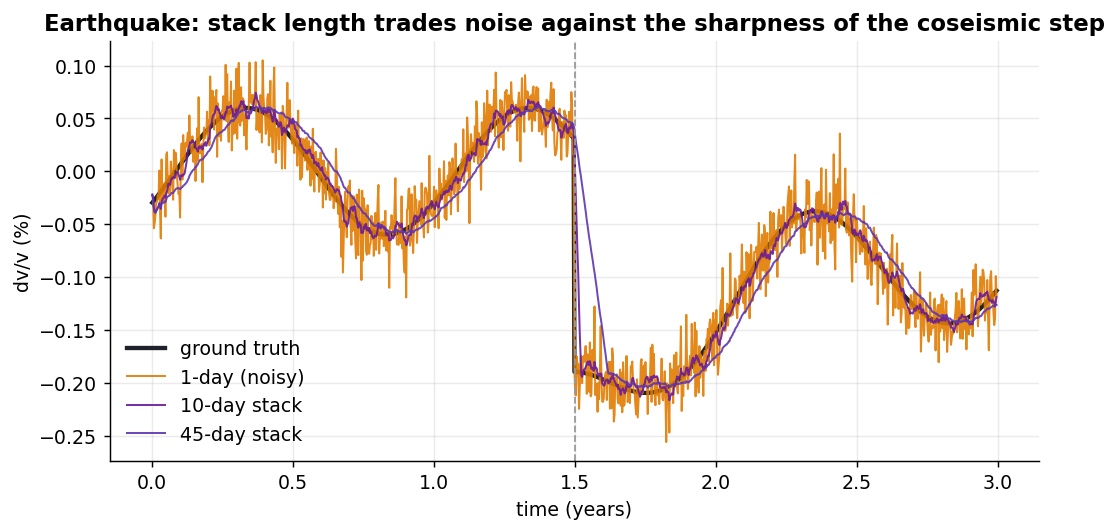
\includegraphics[width=0.49\textwidth]{demo_6_stacking.png}
  \caption{Parameter choices. (a) Frequency band selects depth and signal. (b)
  A coda window does not transfer across bands. (c) Reference strategy: a moving
  reference erases the trend a fixed reference and the joint inversion keep. (d)
  Stacking length smears the coseismic step.}
  \label{fig:params}
\end{figure}

\subsection{Choices that manufacture \dvv, and the multiverse}
\label{sec:artifacts}

Some choices do not merely bias the result --- they fabricate signal. A station
clock error delays the whole correlation by a lapse-independent shift, producing
an apparent \dvv\ that appears with opposite sign on the causal and acausal
branches; measuring the two branches separately is the diagnostic
(Fig.~\ref{fig:artifacts}a). Seasonally varying noise sources warp the low-SNR
late coda, so a late measurement window reports a coherent spurious
\emph{seasonal} \dvv\ many times the real signal while an earlier window stays
clean \citep[the waveform-level version of][]{Zhan2013}
(Fig.~\ref{fig:artifacts}b).

\begin{figure}[t]
  \centering
  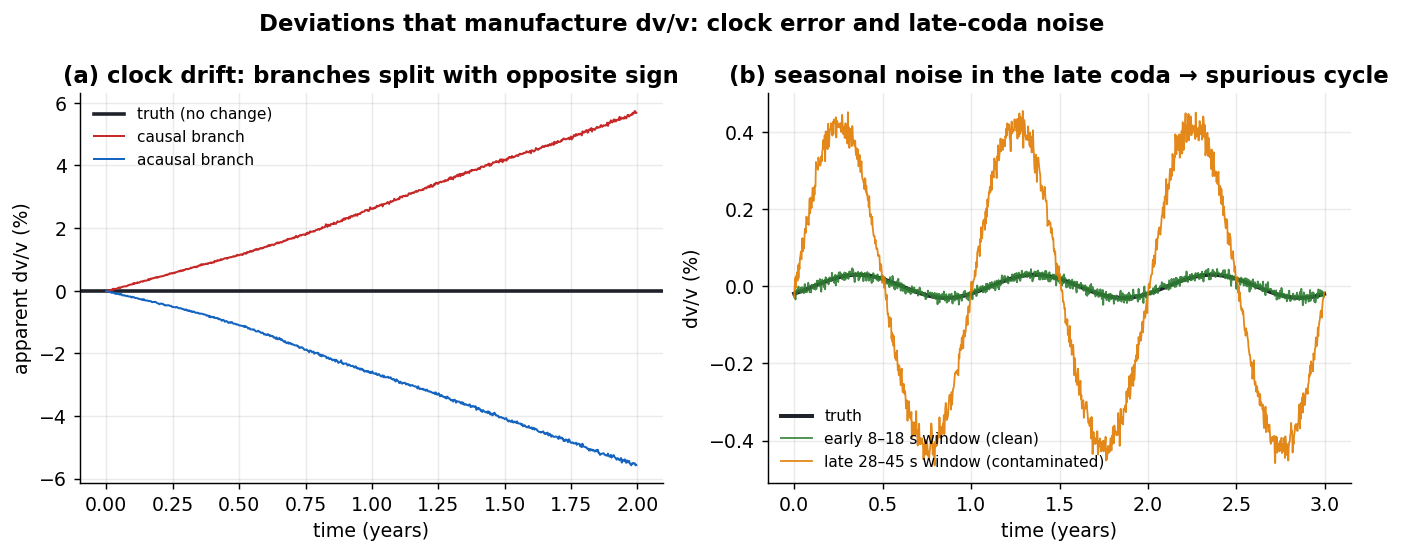
\includegraphics[width=\textwidth]{demo_8_artifacts.png}
  \caption{Deviations that manufacture \dvv. (a) A clock drift splits the causal
  and acausal branches with opposite sign. (b) Seasonal late-coda noise injects a
  spurious seasonal \dvv\ into a late window but not an early one.}
  \label{fig:artifacts}
\end{figure}

Taken together, the choices compound. Running 27 individually defensible
pipelines (three bands $\times$ three windows $\times$ three stack lengths) on one
volcano dataset, the spread across pipelines fans out most exactly where it
matters --- at the sharp co-eruptive drop (Fig.~\ref{fig:multiverse}). The honest
object is therefore a \emph{distribution} of \dvv\ over processing choices, not a
single curve.

\begin{figure}[t]
  \centering
  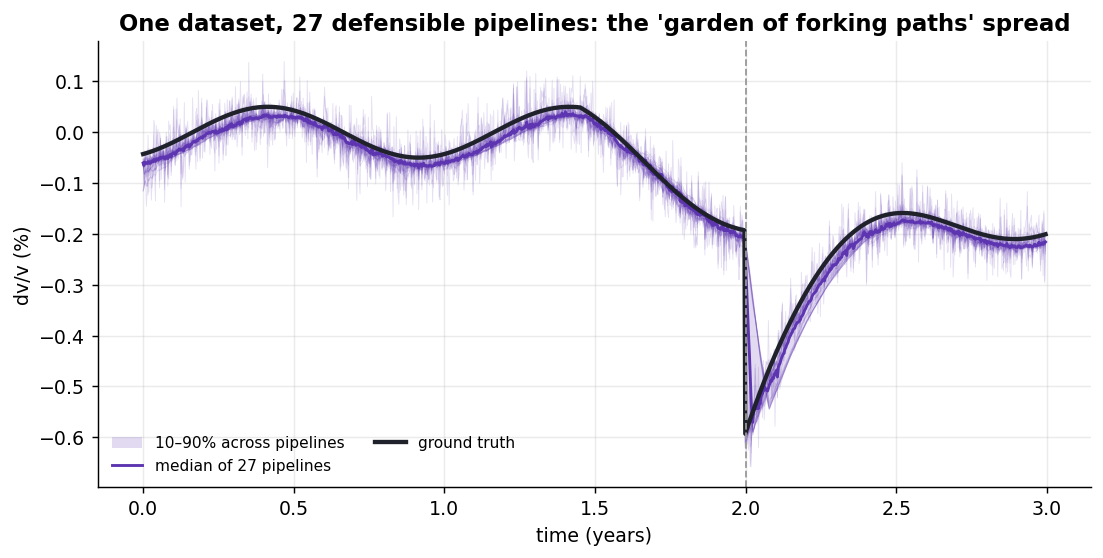
\includegraphics[width=0.8\textwidth]{demo_9_multiverse.png}
  \caption{One dataset, 27 defensible pipelines. The median tracks the truth; the
  10--90\% inter-pipeline spread is largest at the sharp velocity drop.}
  \label{fig:multiverse}
\end{figure}

\section{Discussion}
\label{sec:discussion}

The experiments above share one message: for ambient-noise \dvv, the dominant
control on both the reported value and its uncertainty is frequently the
\emph{processing choice}, not the data. This is uncomfortable but actionable. We
suggest three responses.

\paragraph{Report the choices.} At minimum, a \dvv\ study should state the
estimator and its key parameters, the frequency band(s) and coda window(s) and
how the window was set relative to the band, the reference scheme, the stacking,
the cross-component and station-pair aggregation \emph{and weighting}, and ---
critically --- the exact definition of the quoted uncertainty (within-measurement
error, between-component/pair standard error, or standard deviation). Our results
show that the last item alone can change a stated $1\sigma$ by $\sqrt{N}$.

\paragraph{Quantify the choice-induced uncertainty.} Where a choice is not
forced by the physics, it can be sampled. Pushing a distribution of defensible
processing choices through the measurement-error floors of
\citet{Clarke2011,Weaver2011} yields, by the law of total variance, a marginal
\dvv\ uncertainty that includes the processing-choice spread --- a more honest
error bar than any single pipeline provides, and the natural input to a
depth/stress inversion.

\paragraph{Make it executable.} All synthetics, estimators and figures in this
paper are released in the open \textsc{codameter} package, which reproduces every
result with a single command and is unit-tested. An executable record turns an
undocumented choice into a versioned, inspectable one, and lets a reader re-run a
study's pipeline on the truth-known synthetic to see its bias before trusting it
on data.

\section{Conclusions}
\label{sec:conclusions}

Ambient-noise \dvv\ monitoring rests on a chain of processing choices that are
made ad hoc and reported incompletely. Using a truth-known synthetic and the full
estimator suite of an open toolbox, we have shown that these choices change the
recovered \dvv\ and, more consequentially, change the reported uncertainty by a
factor of $\sim\!\sqrt{N}$ --- enough to flip the significance of a result --- all
without touching the data. The remedy is not a single mandated pipeline but
transparency: report every choice, sample the ones the physics does not fix, and
release the pipeline as executable code. We offer \textsc{codameter} as one such
record.

\section*{Data availability}
The \textsc{codameter} package, including the synthetic-demonstration module, the
figure-generating scripts, and the literature survey that motivates this work, is
openly available at \url{https://github.com/Denolle-Lab/codameter}. All figures
are reproduced by \texttt{python literature/synthetic\_dvv\_demo.py}.

\section*{Acknowledgements}
[To be completed.]

\bibliography{references}

\end{document}
